\documentclass{ximera}

 

\usepackage{epsfig}

\graphicspath{
  {./}
  {figures/}
}

\usepackage{morewrites}
\makeatletter
\newcommand\subfile[1]{%
\renewcommand{\input}[1]{}%
\begingroup\skip@preamble\otherinput{#1}\endgroup\par\vspace{\topsep}
\let\input\otherinput}
\makeatother

\newcommand{\includeexercises}{\directlua{dofile("/home/jim/linearAlgebra/laode/exercises.lua")}}

%\newcounter{ccounter}
%\setcounter{ccounter}{1}
%\newcommand{\Chapter}[1]{\setcounter{chapter}{\arabic{ccounter}}\chapter{#1}\addtocounter{ccounter}{1}}

%\newcommand{\section}[1]{\section{#1}\setcounter{thm}{0}\setcounter{equation}{0}}

%\renewcommand{\theequation}{\arabic{chapter}.\arabic{section}.\arabic{equation}}
%\renewcommand{\thefigure}{\arabic{chapter}.\arabic{figure}}
%\renewcommand{\thetable}{\arabic{chapter}.\arabic{table}}

%\newcommand{\Sec}[2]{\section{#1}\markright{\arabic{ccounter}.\arabic{section}.#2}\setcounter{equation}{0}\setcounter{thm}{0}\setcounter{figure}{0}}

\newcommand{\Sec}[2]{\section{#1}}

\setcounter{secnumdepth}{2}
%\setcounter{secnumdepth}{1} 

%\newcounter{THM}
%\renewcommand{\theTHM}{\arabic{chapter}.\arabic{section}}

\newcommand{\trademark}{{R\!\!\!\!\!\bigcirc}}
%\newtheorem{exercise}{}

\newcommand{\dfield}{{\sf dfield9}}
\newcommand{\pplane}{{\sf pplane9}}

\newcommand{\EXER}{\section*{Exercises}}%\vspace*{0.2in}\hrule\small\setcounter{exercise}{0}}
\newcommand{\CEXER}{}%\vspace{0.08in}\begin{center}Computer Exercises\end{center}}
\newcommand{\TEXER}{} %\vspace{0.08in}\begin{center}Hand Exercises\end{center}}
\newcommand{\AEXER}{} %\vspace{0.08in}\begin{center}Hand Exercises\end{center}}

% BADBAD: \newcommand{\Bbb}{\bf}

\newcommand{\R}{\mbox{$\Bbb{R}$}}
\newcommand{\C}{\mbox{$\Bbb{C}$}}
\newcommand{\Z}{\mbox{$\Bbb{Z}$}}
\newcommand{\N}{\mbox{$\Bbb{N}$}}
\newcommand{\D}{\mbox{{\bf D}}}
\usepackage{amssymb}
%\newcommand{\qed}{\hfill\mbox{\raggedright$\square$} \vspace{1ex}}
%\newcommand{\proof}{\noindent {\bf Proof:} \hspace{0.1in}}

\newcommand{\setmin}{\;\mbox{--}\;}
\newcommand{\Matlab}{{M\small{AT\-LAB}} }
\newcommand{\Matlabp}{{M\small{AT\-LAB}}}
\newcommand{\computer}{\Matlab Instructions}
\newcommand{\half}{\mbox{$\frac{1}{2}$}}
\newcommand{\compose}{\raisebox{.15ex}{\mbox{{\scriptsize$\circ$}}}}
\newcommand{\AND}{\quad\mbox{and}\quad}
\newcommand{\vect}[2]{\left(\begin{array}{c} #1_1 \\ \vdots \\
 #1_{#2}\end{array}\right)}
\newcommand{\mattwo}[4]{\left(\begin{array}{rr} #1 & #2\\ #3
&#4\end{array}\right)}
\newcommand{\mattwoc}[4]{\left(\begin{array}{cc} #1 & #2\\ #3
&#4\end{array}\right)}
\newcommand{\vectwo}[2]{\left(\begin{array}{r} #1 \\ #2\end{array}\right)}
\newcommand{\vectwoc}[2]{\left(\begin{array}{c} #1 \\ #2\end{array}\right)}

\newcommand{\ignore}[1]{}


\newcommand{\inv}{^{-1}}
\newcommand{\CC}{{\cal C}}
\newcommand{\CCone}{\CC^1}
\newcommand{\Span}{{\rm span}}
\newcommand{\rank}{{\rm rank}}
\newcommand{\trace}{{\rm tr}}
\newcommand{\RE}{{\rm Re}}
\newcommand{\IM}{{\rm Im}}
\newcommand{\nulls}{{\rm null\;space}}

\newcommand{\dps}{\displaystyle}
\newcommand{\arraystart}{\renewcommand{\arraystretch}{1.8}}
\newcommand{\arrayfinish}{\renewcommand{\arraystretch}{1.2}}
\newcommand{\Start}[1]{\vspace{0.08in}\noindent {\bf Section~\ref{#1}}}
\newcommand{\exer}[1]{\noindent {\bf \ref{#1}}}
\newcommand{\ans}{}
\newcommand{\matthree}[9]{\left(\begin{array}{rrr} #1 & #2 & #3 \\ #4 & #5 & #6
\\ #7 & #8 & #9\end{array}\right)}
\newcommand{\cvectwo}[2]{\left(\begin{array}{c} #1 \\ #2\end{array}\right)}
\newcommand{\cmatthree}[9]{\left(\begin{array}{ccc} #1 & #2 & #3 \\ #4 & #5 &
#6 \\ #7 & #8 & #9\end{array}\right)}
\newcommand{\vecthree}[3]{\left(\begin{array}{r} #1 \\ #2 \\
#3\end{array}\right)}
\newcommand{\cvecthree}[3]{\left(\begin{array}{c} #1 \\ #2 \\
#3\end{array}\right)}
\newcommand{\cmattwo}[4]{\left(\begin{array}{cc} #1 & #2\\ #3
&#4\end{array}\right)}

\newcommand{\Matrix}[1]{\ensuremath{\left(\begin{array}{rrrrrrrrrrrrrrrrrr} #1 \end{array}\right)}}

\newcommand{\Matrixc}[1]{\ensuremath{\left(\begin{array}{cccccccccccc} #1 \end{array}\right)}}



\renewcommand{\labelenumi}{\theenumi)}
\newenvironment{enumeratea}%
{\begingroup
 \renewcommand{\theenumi}{\alph{enumi}}
 \renewcommand{\labelenumi}{(\theenumi)}
 \begin{enumerate}}
 {\end{enumerate}\endgroup}



\newcounter{help}
\renewcommand{\thehelp}{\thesection.\arabic{equation}}

%\newenvironment{equation*}%
%{\renewcommand\endequation{\eqno (\theequation)* $$}%
%   \begin{equation}}%
%   {\end{equation}\renewcommand\endequation{\eqno \@eqnnum
%$$\global\@ignoretrue}}

%\input{psfig.tex}

\author{Martin Golubitsky and Michael Dellnitz}

%\newenvironment{matlabEquation}%
%{\renewcommand\endequation{\eqno (\theequation*) $$}%
%   \begin{equation}}%
%   {\end{equation}\renewcommand\endequation{\eqno \@eqnnum
% $$\global\@ignoretrue}}

\newcommand{\soln}{\textbf{Solution:} }
\newcommand{\exercap}[1]{\centerline{Figure~\ref{#1}}}
\newcommand{\exercaptwo}[1]{\centerline{Figure~\ref{#1}a\hspace{2.1in}
Figure~\ref{#1}b}}
\newcommand{\exercapthree}[1]{\centerline{Figure~\ref{#1}a\hspace{1.2in}
Figure~\ref{#1}b\hspace{1.2in}Figure~\ref{#1}c}}
\newcommand{\para}{\hspace{0.4in}}

\renewenvironment{solution}{\suppress}{\endsuppress}

\ifxake
\newenvironment{matlabEquation}{\begin{equation}}{\end{equation}}
\else
\newenvironment{matlabEquation}%
{\let\oldtheequation\theequation\renewcommand{\theequation}{\oldtheequation*}\begin{equation}}%
  {\end{equation}\let\theequation\oldtheequation}
\fi

\makeatother


\title{m3.tex}

\begin{document}
\begin{abstract}
BADBAD
\end{abstract}
\maketitle

\chapter{Matrices and Linearity}

\subsection*{Section~\protect{\ref{S:4.1}} Matrix Multiplication of Vectors}
\rhead{S:4.1}{MATRIX MULTIPLICATION OF VECTORS}

\exer{c4.1.1}
\[
Ax =
\left(\begin{array}{rr} 2 & 1 \\ -1 & 4\end{array}\right)
\left(\begin{array}{r} 3 \\ -2\end{array}\right) =
\left(\begin{array}{r} 6 - 2 \\ -3 - 8\end{array}\right) =
\left(\begin{array}{r} 4 \\ -11\end{array}\right)
\]

\exer{c4.1.2}
\[
By =
\left(\begin{array}{rrr} 3 & 4 & 1 \\ 1 & 2 & 3\end{array}\right)
\left(\begin{array}{r} 2 \\ 5 \\ -2\end{array}\right) = 
\left(\begin{array}{r} 6 + 20 - 2 \\ 2 + 10 - 6\end{array}\right) =
\left(\begin{array}{r} 24 \\ 6\end{array}\right)
\]

\exer{c4.1.a3a} $Ax = \vectwo{6}{-10}$.

\exer{c4.1.a3b} The product $Ax$ cannot be computed.

\exer{c4.1.a3c} $Ax = \left(13\right)$.

\exer{c4.1.a3d} The product $Ax$ cannot be computed.

\exer{c4.1.b3}
Compute $Ax$ directly:
\[ Ax = \left(\begin{array}{c} x_1a_{11} + x_2a_{12} + \cdots +
x_na_{1n} \\  x_1a_{21} + x_2a_{22} + \cdots + x_na_{2n} \\
\\ \vdots \\ x_1a_{m1} + x_2a_{m2} + \cdots + x_na_{mn}
\end{array}\right) = x_1\left(\begin{array}{r} a_{11} \\ a_{21} \\
\vdots \\ a_{m1} \end{array}\right) + x_2\left(\begin{array}{r}
a_{12} \\ a_{22} \\ \vdots \\ a_{m2} \end{array}\right) + \cdots
+ x_n\left(\begin{array}{r} a_{1n} \\ a_{2n} \\
\vdots \\ a_{mn} \end{array}\right). \]
So, it is indeed true that $Ax = x_1A_1 + x_2A_2 + \cdots
+ x_nA_n$.

\newpage
\exer{c4.1.3}
\ans The equation $Cz = b$ is valid for $z = (\frac{2}{3},\frac{1}{3})^t$.

\soln Let $z = (z_1,z_2)^t$.  Then $Cz = b$ implies
\[
\left(\begin{array}{rr} 1 & 1 \\ 2 & -1\end{array}\right)
\left(\begin{array}{r} z_1 \\ z_2\end{array}\right) =
\left(\begin{array}{r} 1 \\ 1\end{array}\right)
\]
which can be multiplied out, yielding the linear system
\[\begin{array}{rrrrl}
z_1 & + & z_2 & = & 1 \\
2z_1 & - & z_2 & = & 1.\end{array} \]
This system can be solved by substitution to obtain $z_1 =
\frac{2}{3}$ and $z_2 = \frac{1}{3}$.

\exer{c4.1.4}
\[
\left(\begin{array}{rrr} 2 & 3 & -2 \\ 6 & 0 & -5\end{array}\right) 
\left(\begin{array}{r} x_1 \\ x_2 \\ x_3\end{array}\right) = 
\left(\begin{array}{r} 4 \\ 1\end{array}\right)
\]


\exer{c4.1.6}
\ans All solutions are of the form
\[ \left(\begin{array}{r} x_1 \\ x_2 \\ x_3 \\ x_4\end{array}\right) =
\left(\begin{array}{c} \frac{37}{5} - \frac{16}{5}x_3 - \frac{17}{5}x_4 \\
\frac{11}{5} + \frac{7}{5}x_3 - \frac{1}{5}x_4 \\ x_3 \\ x_4\end{array}\right)
\]
where $x_3$ and $x_4$ are free parameters.

\soln Create the augmented matrix
\[ \left(\begin{array}{rrrr|r}
1 & 3 & -1 & 4 & 14 \\
2 & 1 & 5 & 7 & 17 \\
3 & 4 & 4 & 11 & 31\end{array}\right) \]
which can be row reduced to
\[ \left(\begin{array}{rrrr|r}
1 & 0 & \frac{16}{5} & \frac{17}{5} & \frac{37}{5} \\
0 & 1 & -\frac{7}{5} & \frac{1}{5} & \frac{11}{5} \\
0 & 0 & 0 & 0 & 0\end{array}\right), \]
yielding the desired solution.

\exer{c4.1.7} 
\ans The equations are valid when
\[ A = \left(\begin{array}{rr} 3 & 1 \\ -5 & 4\end{array}\right). \]
\soln Let
\[ A = \left(\begin{array}{rr} a_{11} & a_{12} \\ a_{21} & 
a_{22}\end{array}\right). \]
So
\[ \left(\begin{array}{rr} a_{11} & a_{12} \\ a_{21} & a_{22}\end{array}\right)
\left(\begin{array}{r} 1 \\ 0\end{array}\right) =
\left(\begin{array}{r} 3 \\ -5\end{array}\right) \AND
\left(\begin{array}{rr} a_{11} & a_{12} \\ a_{21} & a_{22}\end{array}\right)
\left(\begin{array}{r} 0 \\ 1\end{array}\right) =
\left(\begin{array}{r} 1 \\ 4.\end{array}\right) \]
These matrix equations are equivalent to the linear equations
\[ \begin{array}{rcl}
a_{11} & = & 3 \\
a_{21} & = & -5 \\
a_{12} & = & 1 \\
a_{22} & = & 4.\end{array} \]


\exer{c4.1.8} 
\ans The equations are valid when
\[ A = \left(\begin{array}{rr} 3 & -1 \\ 1 & -2\end{array}\right). \]
\soln Let
\[ A = \left(\begin{array}{rr} a_{11} & a_{12} \\ a_{21} & 
a_{22}\end{array}\right) \]
Then
\[ \left(\begin{array}{rr} a_{11} & a_{12} \\ a_{21} & a_{22}\end{array}\right)
\left(\begin{array}{r} 1 \\ 1\end{array}\right) =
\left(\begin{array}{r} 2 \\ -1\end{array}\right) \AND
\left(\begin{array}{rr} a_{11} & a_{12} \\ a_{21} & a_{22}\end{array}\right)
\left(\begin{array}{r} 1 \\ -1\end{array}\right) =
\left(\begin{array}{r} 4 \\ 3.\end{array}\right) \]
These matrix equations yield the linear system
\[ \begin{array}{rrrrrrrrr}
a_{11} & + & a_{12} & & & & & = & 2 \\
& & & & a_{21} & + & a_{22} & = & -1 \\
a_{11} & - & a_{12} & & & & & = & 4 \\
& & & & a_{21} & - & a_{22} & = & 3, \end{array} \]
which can be written as an augmented matrix and row-reduced to yield
the values $a_{ij}$:
\[ \left(\begin{array}{rrrr|r}
1 & 1 & 0 & 0 & 2 \\
0 & 0 & 1 & 1 & -1 \\
1 & -1 & 0 & 0 & 4 \\
0 & 0 & 1 & -1 & 3\end{array}\right)
\longrightarrow
\left(\begin{array}{rrrr|r}
1 & 0 & 0 & 0 & 3 \\
0 & 1 & 0 & 0 & -1 \\
0 & 0 & 1 & 0 & 1 \\
0 & 0 & 0 & 1 & 2\end{array}\right). \]



\exer{c4.1.9}
\ans There is no $2 \times 2$ upper triangular matrix $A$ that
satisfies equation \Ref{eq:avect}, but any symmetric matrix $A$ of the form
\[ A = \mattwo{1}{2}{2}{a_{22}}, \]
where $a_{22}$ is a real number, satisfies \Ref{eq:avect}.

\soln Let $A$ be the upper triangular matrix
\[ \mattwo{a_{11}}{a_{12}}{0}{a_{22}}. \]
The resulting matrix equation
\[ \mattwo{a_{11}}{a_{12}}{0}{a_{22}}
\vectwo{1}{0} = \vectwo{1}{2} \]
yields the linear equations
\[ \begin{array}{rcl}
a_{11} & = & 1 \\
0 & = & 2.\end{array} \]
The second equation is inconsistent, so there is no solution.

\para Then let $A$ be the symmetric matrix
\[ \mattwo{a_{11}}{a_{12}}{a_{12}}{a_{22}}. \]
Write the matrix equation
\[ \mattwo{a_{11}}{a_{12}}{a_{12}}{a_{22}}
\vectwo{1}{0} = \vectwo{1}{2}, \]
from which we obtain the consistent linear system
\[ \begin{array}{rcl}
a_{11} & = & 1 \\
a_{12} & = & 2.\end{array} \]

\exer{c4.1.a10a} After loading the system into \Matlabp, typing
{\tt b = A*x} yields
\begin{verbatim}
b =
   37.7800
   42.6800
   42.0600
   77.6100
   87.4700
\end{verbatim}

\exer{c4.1.a10b} Load the system into \Matlabp, then type {\tt b = A*x}
to obtain:
\begin{verbatim}
b =
  103.5000
  175.8000
 -296.9000
 -450.1000
  197.4000
  656.6000
  412.4000
\end{verbatim}

\exer{c4.1.10} Using \Matlabp:
\begin{verbatim}
A\b =
    7.1111
   -2.7778
    1.1111
\end{verbatim}

\exer{c4.1.11} Using \Matlabp:
\begin{verbatim}
A\b =
   -2.3828
   -1.0682
    0.1794
\end{verbatim}

\exer{c4.1.12}
\ans The conditions on $A$ are met when
\[ A = \matthree{2.5}{3.5}{-0.5}{7.5}{9.5}{-4.5}{-5.5}{-6.5}{3.5}. \]

\soln Let
\[
A = \matthree{a_{11}}{a_{12}}{a_{13}}{a_{21}}{a_{22}}{a_{23}}{a_{31}}{a_{32}} 
{a_{33}}
\]
Substituting for $A$ in each of the three equations yields:
\[ \begin{array}{c}
\matthree{a_{11}}{a_{12}}{a_{13}}{a_{21}}{a_{22}}{a_{23}}{a_{31}}
{a_{32}} {a_{33}} \vecthree{2}{-1}{1} = \vecthree{1}{1}{-1} \\
\matthree{a_{11}}{a_{12}}{a_{13}}{a_{21}}{a_{22}}{a_{23}}{a_{31}}
{a_{32}} {a_{33}} \vecthree{1}{-1}{0} = \vecthree{-1}{-2}{1} \\
\matthree{a_{11}}{a_{12}}{a_{13}}{a_{21}}{a_{22}}{a_{23}}{a_{31}}
{a_{32}} {a_{33}} \vecthree{0}{2}{4} = \vecthree{5}{1}{1}.\end{array} \]
These equations can be rewritten as the linear system:
\[ \begin{array}{rrrrrrr}
2a_{11} & - & a_{12} & + & a_{13} & = & 1 \\
2a_{21} & - & a_{22} & + & a_{23} & = & 1 \\
2a_{31} & - & a_{32} & + & a_{33} & = & -1 \\
a_{11} & - & a_{12} & & & = & -1 \\
a_{21} & - & a_{22} & & & = & -2 \\
a_{31} & - & a_{32} & & & = & 1 \\
& & 2a_{12} & + & 4a_{13} & = & 5 \\
& & 2a_{22} & + & 4a_{23} & = & 1 \\
& & 2a_{32} & + & 4a_{33} & = & 1 \end{array} \]
We can enter the left-hand side of the system into \Matlab as
matrix {\tt C} and the right-hand side as vector {\tt b}. 
\[ C = \left(\begin{array}{rrrrrrrrr}
2 & -1 & 1 & 0 & 0 & 0 & 0 & 0 & 0 \\
0 & 0 & 0 & 2 & -1 & 1 & 0 & 0 & 0 \\
0 & 0 & 0 & 0 & 0 & 0 & 2 & -1 & 1 \\
1 & -1 & 0 & 0 & 0 & 0 & 0 & 0 & 0 \\
0 & 0 & 0 & 1 & -1 & 0 & 0 & 0 & 0 \\
0 & 0 & 0 & 0 & 0 & 0 & 1 & -1 & 0 \\
0 & 2 & 4 & 0 & 0 & 0 & 0 & 0 & 0 \\
0 & 0 & 0 & 0 & 2 & 4 & 0 & 0 & 0 \\
0 & 0 & 0 & 0 & 0 & 0 & 0 & 2 & 4 \end{array}\right)
\mbox{\hspace{1.0in}}
b = \left(\begin{array}{r}
1 \\ 1 \\ - 1 \\ -1 \\ -2 \\ 1 \\ 5 \\ 1 \\ 1 \end{array}\right). \]
Then solve to obtain:

\begin{verbatim}
C\b =
    2.5000
    3.5000
   -0.5000
    7.5000
    9.5000
   -4.5000
   -5.5000
   -6.5000
    3.5000
\end{verbatim}
Substitute these values back into $A$ to obtain the appropriate matrix.


\subsection*{Section~\protect{\ref{s:4.2}} Matrix Mappings}
\rhead{s:4.2}{MATRIX MAPPINGS}

\exer{c4.2.a1a}
\ans If $x = (x_1,0)^t$, where $x_1$ is any real scalar, then $Ax = 0$.

\soln Let $x = (x_1,x_2)^t$ and solve the system
\[
Ax = \mattwo{0}{1}{0}{-2}\vectwo{x_1}{x_2} = \vectwo{0}{0}
\]
by row reducing $A$ to obtain
\[
\mattwo{0}{1}{0}{0}.
\]
Thus, $Ax = 0$ when $x_2 = 0$.

\exer{c4.2.a1b} \ans  If $x = (-2x_2,x_2)^t$, where $x_2$ is any real
scalar, then $Bx = 0$.

\soln Let $x = (x_1,x_2)^t$, and solve $Bx = 0$ by row reducing $B$:
\[
\mattwo{1}{2}{-2}{-4} \longrightarrow \mattwo{1}{2}{0}{0}.
\]
Therefore, $Bx = 0$ when $x_1 + 2x_2 = 0$.

\exer{c4.2.a1c}
\ans If $x = (x_1,3x_1)^t$, where $x_1$ is any real scalar, then $Cx = 0$.

\soln Solve $Cx = 0$ by row reducing $C$ to find that $Cx = 0$ when
$x_1 - \frac{1}{3}x_2 = 0$.

\exer{c4.2.1a} \ans
\[ R_{30^\circ} = \mattwo{\cos 30^\circ}{-\sin 30^\circ}
{\sin 30^\circ}{\cos 30^\circ} =
\mattwo{\frac{\sqrt{3}}{2}}{-\frac{1}{2}}{\frac{1}{2}}{\frac{\sqrt{3}}{2}}.
\]

\soln The $2\times 2$ matrix that rotates the plane counterclockwise
through an angle $\theta$ is
\[
R_{\theta} = \mattwo{\cos \theta}{-\sin \theta}{\sin \theta}{\cos \theta}.
\]

\newpage
\exer{c4.2.1b} \ans
\[
R_{(-45^\circ)} = \mattwo{\cos (-45^\circ)}{-\sin
(-45^\circ)}{\sin (-45^\circ)}{\cos (-45^\circ)} =
\mattwo{\frac{1}{\sqrt{2}}}{\frac{1}{\sqrt{2}}}{-\frac{1}{\sqrt{2}}}
{\frac{1}{\sqrt{2}}}.
\]

\exer{c4.2.1c} \ans
\[
2R_{(-90^\circ)} = \mattwo{2\cos (-90^\circ)}{-2\sin
(-90^\circ)}{2\sin (-90^\circ)}{2\cos (-90^\circ)} = \mattwo{0}{2}{-2}{0}.
\]

\exer{c4.2.2a} The map $L_A$ that reflects vectors across the $x$-axis is
$(x,y) \rightarrow (x,-y)$.  The matrix is
\[
A = \mattwo{1}{0}{0}{-1}.
\]

\exer{c4.2.2b} The map $L_A$ that reflects vectors across the $y$-axis is
$(x,y) \rightarrow (-x,y)$.  The matrix is
\[
A = \mattwo{-1}{0}{0}{1}.
\]

\exer{c4.2.2c} The map $L_A$ that reflects vectors across the line $y=x$ is
$(x,y) \rightarrow (y,x)$.  The matrix is
\[
A = \mattwo{0}{1}{1}{0}.
\]

\exer{c7.8.1}
For any point $(x,y)$ in the plane, $A(x,y)^t = (x + Ky,y)^t$.  Therefore,
if $K > 0$, then $(x,y)$ is shifted to the right by a factor of $Ky$.  If
$K < 0$, then $(x,y)$ is shifted to the left by a factor of $|K|y$.  If
$K = 0$, then $(x,y)$ is mapped to itself.

\exer{c7.8.2}
\ans The matrix
\[ R_{90^\circ} = \mattwo{\cos{90^\circ}}{-\sin{90^\circ}}
{\sin{90^\circ}}{\cos{90^\circ}} = \mattwo{0}{-1}{1}{0} \]
performs the desired transformation.

\soln Note that the transformations $(3,4) \rightarrow (-4,3)$ and
$(1,-2) \rightarrow (2,1)$ are obtained by rotating the plane
$90^\circ$ counterclockwise.  Then use \Ref{e:rotmat} to obtain the
matrix corresponding to this rotation.

\exer{c4.2.3}
\ans The matrix is
\[ P = \left(\begin{array}{rrr} 1 & 0 & 0 \\ 0 & 1 & 0\end{array}\right). \]

\soln Let
\[ P = \left(\begin{array}{rrr} p_{11} & p_{12} & p_{13} \\
p_{21} & p_{22} & p_{23}\end{array}\right). \]
Note that a matrix that projects $xyz$ space onto the $xy$ plane
satisfies the vector equations:
\[ \begin{array}{c} \left(\begin{array}{rrr} p_{11} & p_{12} &
p_{13} \\ p_{21} & p_{22} & p_{23} \end{array}\right)
\vecthree{1}{0}{0} = \vectwo{1}{0} \\
\left(\begin{array}{rrr} p_{11} & p_{12} & p_{13} \\ p_{21} &
p_{22} & p_{23} \end{array}\right) \vecthree{0}{1}{0} = \vectwo{0}{1} \\
\left(\begin{array}{rrr} p_{11} & p_{12} & p_{13} \\ p_{21} & p_{22}
& p_{23} \end{array}\right) \vecthree{0}{0}{1} = \vectwo{0}{0} \end{array} 
\]
from which we get the equations
\[ \begin{array}{rrrrrrr}
p_{11} & = & 1 \\
p_{21} & = & 0 \end{array},
\quad
\begin{array}{rrrrrrr}
p_{12} & = & 0 \\
p_{22} & = & 1 \end{array}
\AND
\begin{array}{rrrrrrr}
p_{13} & = & 0 \\
p_{23} & = & 0 \end{array}. 
\]
Substitute these values back into $P$ to obtain the solution.

\exer{c4.2.3a} The matrix which is a rotation of the plane 
through angle $\theta$ followed by a dilatation $cI_2$ is
\[
cR_\theta =
\mattwo{c\cos\theta}{-c\sin\theta}{c\sin\theta}{c\cos\theta}.
\]
In order for the given matrix to equal $cR_\theta$, we need
\[
\mattwo{a}{-b}{b}{a} =
\mattwo{c\cos\theta}{-c\sin\theta}{c\sin\theta}{c\cos\theta}.
\]
Thus, we have $a = c\cos\theta$ and $b = c\sin\theta$.  We can then write
\[
c^2 = c^2(cos^2\theta + \sin^2\theta) = c^2\cos^2\theta + c^2\sin^2\theta
= a^2 + b^2,
\]
or
\[
c = \sqrt{a^2 + b^2}.
\]

\exer{c4.2.3b} \ans This matrix is a counterclockwise rotation through an 
angle $\theta = \sin^{-1}\left(\frac{-4}{5}\right) \approx 2\pi-0.9273
\approx 5.3559$ and a dilatation by a scalar $c = 5$.

\soln This follows from Exercise~\ref{c4.2.3a} with $a = 3$
and $b = -4$.  Thus, $c = \sqrt{a^2 + b^2} = 5$ and
$\theta = \sin^{-1}\left(\frac{b}{\sqrt{a^2 + b^2}}\right) = 
\sin^{-1}\left(\frac{-4}{5}\right)$.  Add $2\pi$ to correspond to counterclockwise rotation.

\exer{c4.2.a4a} The matrix $A$ maps any vector $x$ of the form
$x = s(1,1)^t$, where $s$ is a real scalar, to twice its length, and any
vector of the form $x = s(0,1)^t$ to half its length.

\para If you are having trouble finding this vector with {\tt map},
turn on the rescale vectors option, which scales every vector to length
$1$ after mapping it.  Then, test vectors by applying {\sf map} several
times until you find a vector which (approximately) maps to itself.

\newpage
\exer{c4.2.a4b} The matrix $B$ maps any vector of the form
$x \approx s(-0.89,0.46)$ to approximately $1.97$ times its length.

\exer{c4.2.a4c} The matrix $C$ maps any vector of the form $x = s(1,0)$
to twice its length and maps any vector of the form $x = s(1,2)$ to
$-\frac{1}{2}$ times its length.

\exer{c4.2.ba} \ans Matrix $A$ rotates the plane by $\theta =
\approx 1.1071$ counterclockwise and dilatates it by a factor of
$c = \sqrt{5} \approx 2.2361$.

\soln Matrix $A$ is a special case of Exercise~\ref{c4.2.3a} with $a = 1$
and $b = 2$.  Thus, $c = \sqrt{a^2 + b^2} = \sqrt{5}$ and
$\theta = \cos^{-1}\left(\frac{a}{\sqrt{a^2 + b^2}}\right) =
\cos^{-1}\left(\frac{1}{\sqrt{1^2 + 2^2}}\right) \approx 1.1071$.

\exer{c4.2.bb} \ans Matrix $B$ rotates the plane by $\theta =
\approx 3.0585$ counterclockwise and dilatates it by a factor of
$c = \sqrt{5.8} \approx 2.4083$.

\soln Matrix $B$ is a special case of Exercise~\ref{c4.2.3a} with $a = -2.4$
and $b = 0.2$.  Thus, $c = \sqrt{a^2 + b^2} = \sqrt{5.8}$ and
$\theta = \cos^{-1}\left(\frac{a}{\sqrt{a^2 + b^2}}\right) =
\cos^{-1}\left(-\frac{2.4}{\sqrt{(-2.4)^2 + (0.2)^2}}\right) \approx 3.0585$.

\exer{c4.2.bc} \ans Matrix $C$ rotates the plane by $\theta =
\approx 0.4531$ counterclockwise and dilatates it by a factor of
$c \approx 2.9697$.

\soln Matrix $C$ is a special case of Exercise~\ref{c4.2.3a} with $a = 2.67$
and $b = -1.3$.  Thus, $c = \sqrt{a^2 + b^2} = \sqrt{(2.67)^2 + (-1.3)^2}
\approx 2.9697$ and
\[
\theta = \cos^{-1}\left(\frac{a}{\sqrt{a^2 + b^2}}
\right) = \cos^{-1}\left(\frac{2.67}{\sqrt{(2.67)^2 + (-1.3)^2}}\right)
\approx 0.4531.
\]

\exer{c4.2.4a} $A$ rotates the plane $30^\circ$ clockwise.

\exer{c4.2.4b} $B$ rotates the plane $45^\circ$ counterclockwise and
reduces it by a factor of $\sqrt{2}$.

\exer{c4.2.4c} $C$ reflects the plane across the line $y = x$.

\exer{c4.2.4d} $D$ maps the plane onto the $x$-axis.

\exer{c4.2.4e} $E$ maps $(x,y)$ to a point on the line $y = x$; that
point is $(\frac{x + y}{2}, \frac{x + y}{2})$.


\exer{c4.2.5}  Both matrices map the dog to the point $(-1,-1)$ but the
orientation of the dog is different in the two cases.  See 
Figure~\ref{c4.2.5}.
\begin{figure}[htb]
     \centerline{%
     \psfig{file=exfigure/fig3-2-26a.eps,width=3.0in}
     \psfig{file=exfigure/fig3-2-26b.eps,width=3.0in}}
        \exercaptwo{c4.2.5}
\end{figure} 


\subsection*{Section~\protect{\ref{S:linearity}} Linearity}
\rhead{S:linearity}{LINEARITY}

\exer{c4.3.1}
(a) $2(2,4) - 3(3,-1) = (-5,11)$;

(b) $10(1,0,-1) - 2(2,-4,3) = (6,8,-16)$;

(c) $5(4,2,-1,1) - 1(-1,3,5,7) = (21,7,-10,-2)$.

\exer{c4.3.2}
$\alpha (4,7) + \beta (2,-1) = (4\alpha + 2\beta, 7\alpha - \beta)$.

\exer{c4.3.3}
The equation
\[ (-2, -1) = \alpha(1,2) + \beta(1,-3) =
(\alpha + \beta, 2\alpha - 3\beta ) \]
can be rewritten as the linear system
\[ \begin{array}{rrrrr}
-2 & = & \alpha & + & \beta \\
-1 & = & 2\alpha & - & 3\beta\end{array}. \]
Solving this system yields $\alpha = -\frac{7}{5}$ and
$\beta = -\frac{3}{5}$.

\exer{c4.3.4}
\ans The vector $z = (2,3,-1)$ cannot be written as
\[
z = \alpha(2,3,0) + \beta(1,-1,1).
\]

\soln Write the equation
\[ (2,3,-1) = \alpha(2,3,0) + \beta(1,-1,1) = 
(2\alpha + \beta, 3\alpha - \beta, \beta) \]
as a linear system of two unknowns in three equations:
\[ \begin{array}{rrrrr}
2 & = & 2\alpha & + & \beta \\
3 & = & 3\alpha & - & \beta \\
-1 & = & \beta \end{array}. \]
Substituting $\beta = -1$ into the first and second equations
yields
\[ \begin{array}{rcl}
\frac{3}{2} & = & \alpha \\
\frac{2}{3} & = & \alpha. \end{array} \]
The system is inconsistent, so there is no solution to the desired
equation.

\exer{c4.3.5}
\ans The equation
\[ \alpha(3,-2) + \beta(2,3) + \gamma(1,4) = (1,-2) \]
holds for any real numbers $\alpha$,$\beta$,
$\gamma$ such that $\alpha = \frac{5}{13}\gamma +
\frac{7}{13}$ and $\beta = -\frac{14}{13}\gamma
- \frac{4}{13}$.

\soln Write the equation as the linear system
\[ \begin{array}{rrrrrrl}
3\alpha & + & 2\beta & + & \gamma & = & 1 \\
-2\alpha & + & 3\beta & + & 4\gamma & = & -2. \end{array} \]
The augmented matrix
\[ \left(\begin{array}{rrr|r}
3 & 2 & 1 & 1 \\
-2 & 3 & 4 & -2 \end{array}\right) \]
row reduces to
\[ \left(\begin{array}{rrr|r}
1 & 0 & -\frac{5}{13} & \frac{7}{13} \\
0 & 1 & \frac{14}{13} & -\frac{4}{13} \end{array}\right) \]
and the equation is valid for any values of $\alpha$,$\beta$,
and $\gamma$ that satisfy this system.

\exer{c4.3.6a} \ans The transformation $T(x,y,z) = (x + 2y - z, x - 4z)$
is linear.

\soln Use the definition that a mapping is linear if it satisfies
\Ref{sum} and \Ref{product} to verify:

\para Let $X_1 = (x_1,y_1,z_1)$ and let $X_2 = (x_2,y_2,z_2)$.
Verify \Ref{sum} by computing $T(X_1 + X_2)$ and comparing it
to $T(X_1) + T(X_2)$.
\[ \begin{array}{rcl}
T(X_1 + X_2) & = & T((x_1,y_1,z_1) + (x_2, y_2, z_2)) \\
& = & T(x_1 + x_2, y_1 + y_2, z_1 + z_2) \\
& = & ((x_1 + x_2) + 2(y_1 + y_2) - (z_1 + z_2),
(x_1 + x_2) - 4(z_1 + z_2)) \\ & = &
(x_1 + x_2 + 2y_1 + 2y_2 - z_1 - z_2, x_1 + x_2 - 4z_1 - 4z_2) \\
& = & (x_1 + 2y_1 - z_1, x_1 - 4z_1) +
(x_2 + 2y_2 - z_2, x_2 - 4z_2). \end{array} \]
\[ \begin{array}{rcl}
T(X_1) + T(X_2)
& = & T(x_1,y_1,z_1) + T(x_2,y_2,z_2) \\
& = & (x_1 + 2y_1 - z_1, x_1 - 4z_1) +
(x_2 + 2y_2 - z_2, x_2 - 4z_2). \end{array} \]
Let $X = (x,y,z)$ and let $c$ be any real scalar.  Verify
\Ref{product} by computing $cT(X)$ and comparing it to $T(cX)$.
\[ \begin{array}{rcl}
cT(X) & = & cT(x,y,z) \\
& = & c(x + 2y - z, x - 4z) \\
& = & (cx + 2cy - cz, cx - 4cz). \end{array} \]
\[ \begin{array}{rcl}
T(cX) & = & T(cx,cy,cz) \\
& = & T(cX) \\
& = & (cx + 2cy - cz, cx - 4cz). \end{array} \]
So $T(x,y,z) = (x + 2y - z, x - 4z)$ is a linear mapping.

\exer{c4.3.6b} \ans The transformation $T(x,y) = (x + xy, 2y)$ is not linear.

\soln If $T$ is a linear transformation, then
\[
T(x_1 + x_2,y_1 + y_2) = T(x_1,y_1) + T(x_2,y_2)
\]
for any real numbers $x_1$,$x_2$,$y_1$,$y_2$.  However,
\[
\begin{array}{rcl}
T(1,1) & = & (2,2) \\
T(1,0) + T(0,1) & = & (1,0) + (0,2) = (1,2).\end{array}
\]
Therefore $T(1,1) \neq T(1,0) + T(0,1)$ and $T$ is not linear.

\exer{c4.3.6c} The transformation $T(x,y) = (x + y, x - y - 1)$
is not linear because $T(0,0) = (0,-1) \neq 0$, contradicting
Theorem~\ref{lin-matrices}.

\exer{c4.3.6d} The transformation $T(x,y) = (1,x + y, 2y)$ is not linear
because $T(0,0) = (1,0,0) \neq 0$.

\exer{c4.3.7}
\ans The matrix that satisfies these conditions is
\[
A = \left(\begin{array}{rrr} 2 & 1 & 0 \\ 3 & -1 & 1
\end{array}\right).
\]

\soln Let
\[
A = \left(\begin{array}{rrr}
a_{11} & a_{12} & a_{13} \\ a_{21} & a_{22} & a_{23}
\end{array}\right).
\]
Rewrite the conditions on $A$ as:
\[
\left(\begin{array}{rrr}
a_{11} & a_{12} & a_{13} \\ a_{21} & a_{22} & a_{23}
\end{array}\right) \vecthree{1}{0}{0} = \vectwo{2}{3}
\]
\[
\left(\begin{array}{rrr}
a_{11} & a_{12} & a_{13} \\ a_{21} & a_{22} & a_{23}
\end{array}\right) \vecthree{0}{1}{0} = \vectwo{1}{-1}
\]
\[
\left(\begin{array}{rrr}
a_{11} & a_{12} & a_{13} \\ a_{21} & a_{22} & a_{23}
\end{array}\right) \vecthree{0}{0}{1} = \vectwo{0}{1}
\]
These equations imply:
\[ \begin{array}{rcl} a_{11} & = & 2 \\ a_{21} & = & 3 \end{array},
\quad
\begin{array}{rcr} a_{12} & = & 1 \\ a_{22} & = & -1 \end{array}
\AND
\begin{array}{rcl} a_{13} & = & 0 \\ a_{23} & = & 1 \end{array}
\]
and determine the matrix $A$.

\exer{c4.3.8}
\ans The matrix of linear mapping $L$ is
\[
A = \matthree{0}{-1}{-1}{1}{0}{2}{1}{-2}{0}.
\]

\soln Let $X = (x_1,x_2,x_3)$ and let $Y = (y_1,y_2,y_3)$.  
Since $K = (2,1,-1)$,
\[
L(X) = (x_1,x_2,x_3) \times K = 
(-x_2 - x_3, x_1 + 2x_3, x_1 - 2x_2).
\]

To show that $L(X)$ is a linear mapping, first demonstrate that
\Ref{sum} is valid:
\[
\begin{array}{rcl}
L(X + Y) & = & L(x_1 + y_1,x_2 + y_2,x_3 + y_3) \\
& = & (-(x_2 + y_2) - (x_3 + y_3), (x_1 + y_1) + 2(x_3 + y_3),
(x_1 + y_1) - 2(x_2 + y_2)) \\
& = & (-x_2 - x_3, x_1 + 2x_3, x_1 - 2x_2) +
(-y_2 - y_3, y_1 + 2y_3, y_1 - 2y_2) \\
& = & L(X) + L(Y), \end{array}
\]
then show that \Ref{product} is valid:
\[
\begin{array}{rcl}
cL(X) & = & cL(x_1,x_2,x_3) \\
& = & c(-x_2 - x_3, x_1 + 2x_3, x_1 - 2x_2) \\
& = & (-cx_2 - cx_3, cx_1 + 2cx_3, cx_1 - 2cx_2) \\
& = & L(cx_1,cx_2,cx_3) \\
& = & L(cX). \end{array}
\]

Find $A$ by noting that $L(e_j) = Ae_j$ is the $j^{th}$ column of $A$,
and computing
\[ \begin{array}{l}
L(e_1) = L(1,0,0) = (0,1,1) \\
L(e_2) = L(0,1,0) = (-1,0,-2) \\
L(e_3) = L(0,0,1) = (-1,2,0). \end{array} \]


\exer{c4.3.9}
To see that $L(X + Y) = L(X) + L(Y)$, consider $X$ and $Y$ as
vectors.  These vectors are two sides of a parallelogram with
diagonal $X + Y$, as shown in Figure~\ref{c4.3.9}a.  Rotating
the plane $45^\circ$ counterclockwise has the effect of
rotating the entire parallelogram, as in Figure~\ref{c4.3.9}b.
Therefore, adding $X$ and $Y$ and then rotating the sum
$X + Y$ is the same as rotating $X$ and $Y$ separately and
then adding them.

\para To see that $cL(X) = L(cX)$, note that multiplying a
vector $X$ by a scalar $c$ affects only the length of the vector,
and that rotating the plane affects only the orientation of
the vector.  Therefore, the two operations can be performed in
either order with the same effect.

\para To find the matrix $A$ of this transformation, we can use
\Ref{e:rotmat}:
\[ A = \mattwo{\cos 45^\circ}{-\sin 45^\circ}{\sin 45^\circ}{\cos 45^\circ}
= \mattwo{\frac{1}{\sqrt{2}}}{-\frac{1}{\sqrt{2}}}
{\frac{1}{\sqrt{2}}}{\frac{1}{\sqrt{2}}} \]

\begin{figure}[htb]
                       \centerline{%
                       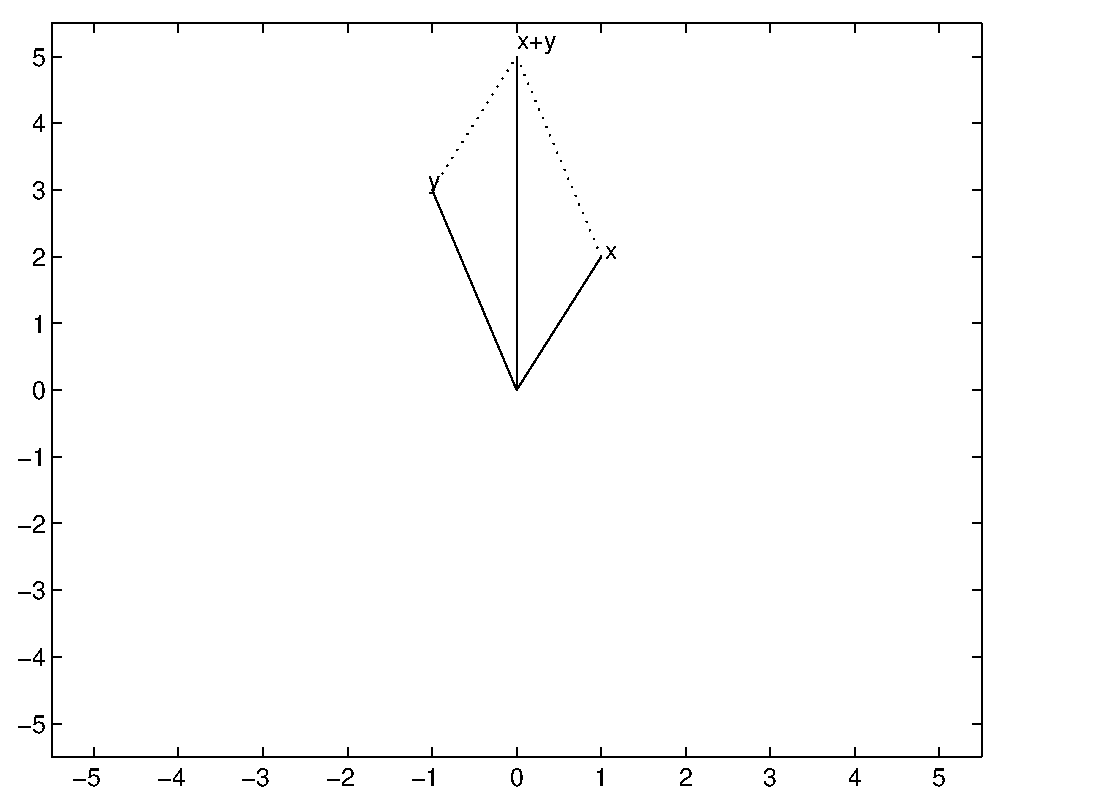
\psfig{file=exfigure/4-3-9a.eps,width=2.75in}
                       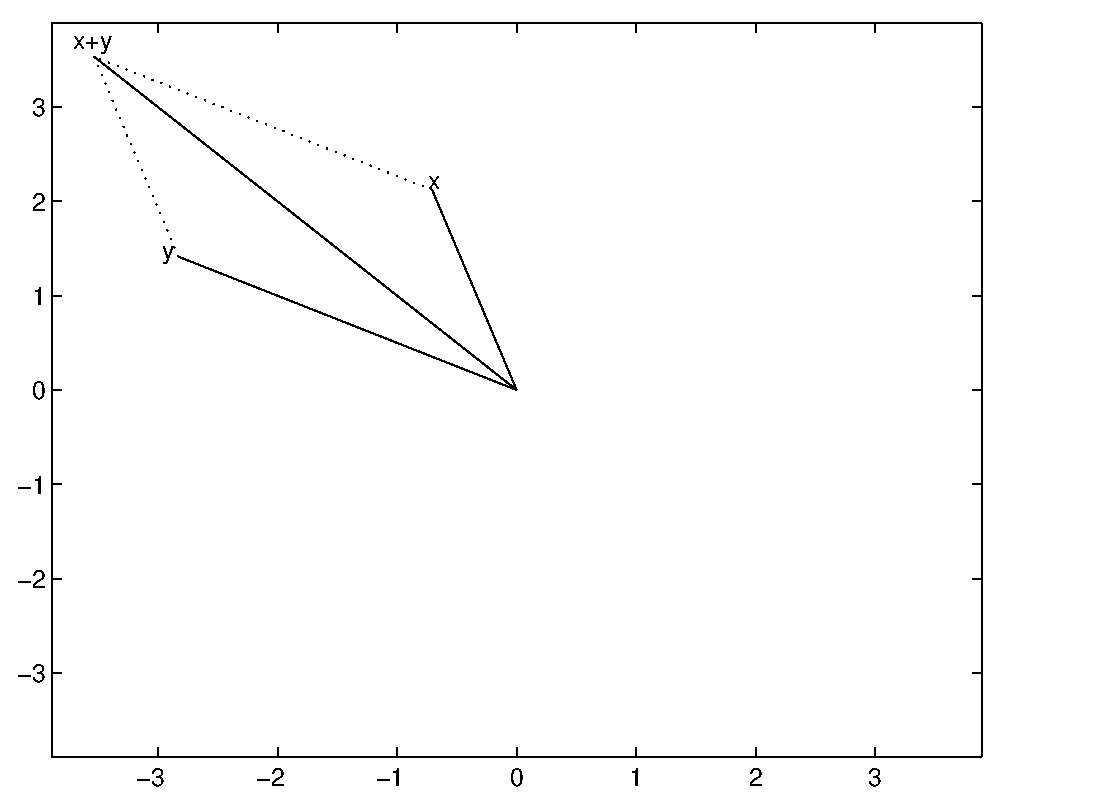
\psfig{file=exfigure/4-3-9b.eps,width=2.75in}}
                \exercaptwo{c4.3.9}
\end{figure}

\exer{c4.3.10}
\ans The matrix of linear mapping $L_A$ is
\[ A = \matthree{0}{1}{0}{0}{0}{1}{1}{0}{0}. \]

\soln Note that if $\sigma = L_A$, then $\sigma(e_j) = Ae_j$ is the
$j^{th}$ column of matrix $A$.  Thus $A$ is determined by
\[
\begin{array}{l}
\sigma(e_1) = \sigma(1,0,0) = (0,0,1) \\
\sigma(e_2) = \sigma(0,1,0) = (1,0,0) \\
\sigma(e_3) = \sigma(0,0,1) = (0,1,0). \end{array}
\]


\exer{c4.3.11}
Let $L(0) = K$.
By the definition of linearity, for any real number $c$,
\[ L(0) = L(c0) = cL(0) \]
which is valid only when $L(0) = 0$.

\exer{c4.3.12}
The mapping $L(x)$ is linear if $L(x + y) = L(x) + L(y)$ and
if $cL(x) = L(cx)$.  We can use the assumption that $L_1(x)$
and $L_2(x)$ are linear mappings to show:
\[ \begin{array}{rcl}
L(x + y) & = & L_1(x + y) + L_2(x + y) \\
& = & L_1(x) + L_1(y) + L_2(x) + L_2(y) \\
& = & [L_1(x) + L_2(x)] + [L_1(y) + L_2(y)] \\
& = & L(x) + L(y) \end{array} \]
and
\[ \begin{array}{rcl}
cL(x) & = & cL_1(x) + cL_2(x) \\
& = & L_1(cx) + L_2(cx) \\
& = & L(cx). \end{array} \]

Assume that $L = L_A$, $L_1 = L_{A_1}$ and $L_2 = L_{A_2}$ for
$m \times n$ matrices $A$, $A_1$, $A_2$.  We claim that
$A = A_1 + A_2$, where $A_1 + A_2$ is the matrix obtained by
adding corresponding entries of $A_1$ and $A_2$.  By
definition, $L(e_j) = L_1(e_j) + L_2(e_j)$.  Lemma~\ref{columnsA}
implies that the $j^{th}$ column of $A$ is the sum of the
$j^{th}$ columns of $A_1$ and $A_2$ for all columns {j}, so
$A = A_1 + A_2$.

\exer{c4.3.13}  Computer experiment.

\exer{c4.3.14}
The mapping $L_A$ performs the transformation $(x,y) \rightarrow
(0.5y, -0.5x)$.  That is, the mapping rotates a 2-vector
$90^\circ$ clockwise then halves its length.

\exer{c4.3.15A} Verify \Ref{sum} by typing {\tt A*(x + y)} to obtain:
\begin{verbatim}
ans =
    24
   -21
    21
\end{verbatim}
Then, type {\tt A*x + A*y}, which yields the same answer.
Verify \Ref{product} by typing {\tt c*(A*x)}, which gives
the same answer as {\tt A*(c*x)}, namely:
\begin{verbatim}
ans =
    84
    84
   231
\end{verbatim}

\exer{c4.3.15B} Typing either {\tt A*(x + y)} or {\tt A*x + A*y} yields
\begin{verbatim}
ans =
   -19
   -15
    24
     3
    15
\end{verbatim}
verifying \Ref{sum}.  Typing {\tt c*(A*x)} or {\tt A*(c*x)} yields
\begin{verbatim}
ans =
  -156
  -364
  -455
  -273
  -117
\end{verbatim}
verifying \Ref{product}.



\subsection*{Section~\protect{\ref{S:Superposition}} The Principle of
Superposition}
\rhead{S:Superposition}{THE PRINCIPLE OF SUPERPOSITION}

\exer{c4.4.1}
(a) \ans All solutions can be written as a superposition of the vectors
\[
v_1 = \vecthree{-1}{1}{0} \AND v_2 = \vecthree{-1}{0}{1}.
\]

\soln The equation $x + y + z = 0$ is a linear system of three variables
in one equation.  If we consider $y$ and $z$ to be free variables, then
every solution to the system has the form
\[
\vecthree{x}{y}{z} = \left(\begin{array}{c} -y - z \\ y \\
z \end{array}\right) = y\vecthree{-1}{1}{0} +
z\vecthree{-1}{0}{1}.
\]

(b) \ans All solutions can be written as a superposition
of the second pair of vectors
\[
w_1 = \vecthree{1}{0}{-1} \AND w_2 = \vecthree{0}{1}{-1}.
\]

\soln Write the same linear system, but this time consider $x$ and $y$
to be free variables.  In this case, every solution has the form:
\[
\vecthree{x}{y}{z} = \left(\begin{array}{c} x \\ y \\
-x - y \end{array}\right) = x\vecthree{1}{0}{-1} +
z\vecthree{0}{1}{-1}.
\]

\exer{c4.4.2}
\ans Every solution can be written as a superposition of the vectors
\[
\left(\begin{array}{r} -2 \\ 1 \\ 0 \\ 0 \\ 0\end{array}\right), \quad
\left(\begin{array}{r} -1 \\ 0 \\ 2 \\ 1 \\ 0 \end{array}\right) \AND
\left(\begin{array}{r} 1 \\ 0 \\ -1 \\ 0 \\ 1 \end{array}\right).
\]

\soln Write the matrix of the homogeneous system:
\[
\left(\begin{array}{rrrrr} 1 & 2 & 0 & 1 & -1 \\
0 & 0 & 1 & -2 & 1 \end{array}\right).
\]
This matrix cannot be row reduced further.  Every solution has the form
\[
\left(\begin{array}{r} x_1 \\ x_2 \\ x_3 \\ x_4 \\ x_5
\end{array}\right) = \left(\begin{array}{c} x_5 - x_4 - 2x_2 \\
x_2 \\ -x_5 + 2x_4 \\ x_4 \\ x_5 \end{array}\right) = 
x_2\left(\begin{array}{r} -2 \\ 1 \\ 0 \\ 0 \\ 0
\end{array}\right) + x_4\left(\begin{array}{r} -1 \\ 0 \\ 2 \\
1 \\ 0 \end{array}\right) + x_5\left(\begin{array}{r} 1 \\ 0 \\
-1 \\ 0 \\ 1 \end{array}\right).
\]

\exer{c4.4.3}
(a) \ans All solutions to the homogeneous equation are of the form
\[
x = \vecthree{x_1}{x_2}{x_3} = s\vecthree{-11}{7}{1}.
\]

\soln Row reduce the matrix of the homogeneous system
$Ax = 0$ to obtain:
\[
\left(\begin{array}{rrr} 1 & 0 & 11 \\ 0 & 1 & -7 \end{array}\right).
\]
So $x_1 = -11s$, $x_2 = 7s$ and $x_3 = s$.

(b) \ans One possible solution is
\[ \vecthree{x_1}{x_2}{x_3} = \vecthree{1}{1}{1}. \]

\soln Assign a value to $x_3$, then substitute into the two equations
of the inhomogeneous system to obtain values for $x_1$ and $x_2$.

(c) All solutions to \Ref{E:inhom} can be found by adding a
single solution of the inhomogeneous system to all solutions
of the homogeneous system, so:
\[
x = \vecthree{1}{1}{1} + s\vecthree{-11}{7}{1}.
\]



\newpage
\subsection*{Section~\protect{\ref{S:4.6}} Composition and Multiplication
of Matrices}
\rhead{S:4.6}{COMPOSITION AND MULTIPLICATION OF MATRICES}

\exer{c4.6.-1a} $AB=\mattwo{-2}{0}{7}{-1}$ and $BA= \mattwo{-2}{0}{5}{-1}$.

\exer{c4.6.-1b} $AB$ is not defined. $BA=\left(\begin{array}{rrr} 8 &  20 &  0\\
 -4 & -16  &  3\end{array}\right)$


\exer{c4.6.-1c} $AB$ is not defined. $BA$  is not defined.  

\exer{c4.6.-1d} $AB$ is not defined. $BA$  is not defined.


\exer{c4.6.0a}
$\mattwo{2}{3}{0}{1}\mattwo{-1}{1}{-3}{2} =
\cmattwo{-2 - 9}{2+6}{-3}{2} = \mattwo{-11}{8}{-3}{2}$.

\exer{c4.6.0b}
$\left(\begin{array}{rrr} 1 & 2 & 3\\ -2 & 3 & -1 \end{array}\right)
\left(\begin{array}{rr} 2 & 3\\ -2 & 5 \\1 & -1 \end{array}\right)
= \mattwo{2 - 4 + 3}{3 + 10 - 3}{-4 - 6 - 1}{-6 + 15 + 1}
= \mattwo{1}{10}{-11}{10}$.

\exer{c4.6.0c} $\left(\begin{array}{rr} 2 & 3\\ -2 & 5 \\1 & -1 \end{array}
\right) \left(\begin{array}{rrr} 1 & 2 & 3\\ -2 & 3 & -1 \end{array}\right)
= \matthree{-4}{13}{3}{-12}{11}{-11}{3}{-1}{4}$.

\exer{c4.6.0d}
$\left(\begin{array}{rrr} 2 &  -1 &3\\ 1 & 0 & 5 \\1 & 5 & -1
\end{array}\right)
\left(\begin{array}{rrr} 1 & 7 \\ -2 & -1 \\ -5 & 3\end{array}\right)
= \left(\begin{array}{cc} 2+2-15 & 14+1+9 \\ 1-25 & 7+15 \\
1-10+5 & 7-5-3 \end{array}\right)
= \left(\begin{array}{rr} -11 & 24 \\ -24 & 22 \\ -4 & -1
\end{array}\right)$.


\exer{c4.6.1}
\ans For any matrix $B$ of the form
\[
\mattwo{b_{11}}{0}{0}{b_{22}}
\]
the equation $AB = BA$ is valid.

\soln Let
\[
B = \mattwo{b_{11}}{b_{12}}{b_{21}}{b_{22}}.
\]
Then compute the matrix $B$ for which
\[
\begin{array}{rcl}
AB & = & BA \\
\mattwo{2}{0}{0}{-1}\mattwo{b_{11}}{b_{12}}{b_{21}}{b_{22}} &
= & \mattwo{b_{11}}{b_{12}}{b_{21}}{b_{22}}\mattwo{2}{0}{0}{-1} \\
\mattwo{2b_{11}}{2b_{12}}{-b_{21}}{-b_{22}} & = &
\mattwo{2b_{11}}{-b_{12}}{2b_{21}}{-b_{22}} \end{array}
\]
which is equivalent to the linear system
\[
\begin{array}{l}
2b_{11} = 2b_{11} \\
2b_{12} = -b_{12} \\
-b_{21} = 2b_{21} \\
-b_{22} = -b_{22}. \end{array}
\]

\exer{c4.6.2}
\ans 
\[
B = \mattwo{\frac{4}{5}}{3}{\frac{3}{5}}{2}.
\]

\soln Compute
\[
\begin{array}{rcl}
AB & = & BA \\
\mattwo{2}{5}{1}{4}\mattwo{a}{3}{b}{2} & = &
\mattwo{a}{3}{b}{2}\mattwo{2}{5}{1}{4} \\
\mattwo{2a+5b}{16}{a+4b}{11} & = & \mattwo{2a+3}{5a+12}{2b+2}{5b+8}.
\end{array}
\]
This equation can be rewritten as the system
\[
\begin{array}{rcl}
2a + 5b & = & 2a + 3 \\
16 & = & 5a + 12 \\
a + 4b & = & 2b + 2 \\
11 & = & 5b + 8 \end{array}
\]
which yields the solution $a = 4/5$ and $b = 3/5$.

\exer{c4.6.3}
\[ AA^t = \matthree{1}{0}{-3}{-2}{1}{1}{0}{1}{-5}
\matthree{1}{-2}{0}{0}{1}{1}{-3}{1}{-5} =
\matthree{10}{-5}{15}{-5}{6}{-4}{15}{-4}{26}. \]



\exer{c4.7.1a}
Load the system into \Matlabp.  The matrix $AB$ is defined,
and typing {\tt A*B} yields:
\begin{verbatim}
ans =
    10     0    -2
   -12     4    16
\end{verbatim}
The matrix $BA$ is not defined, since $B$ has 3 columns while $A$
has 2 rows.  Typing {\tt B*A} generates an error message.

\exer{c4.7.1b} The matrix $AB$ is not defined because $A$ has 5 columns
while $B$ has four rows.  The matrix $BA$ is also not defined
because $B$ has 6 columns and $A$ has 3 rows.

\exer{c4.7.1c} Both $AB$ and $BA$ are defined and can be computed using
\Matlabp :
\begin{verbatim}
A*B                                     B*A
ans =                                   ans =   
   -34   -26     7   -23                    -8     4    -8    35
    -6    19    25    15                    -8    -1    28     3
   -15     6    -5     7                     2    27     0   -43
    -4   -11    12    -6                     7     0     3   -17
\end{verbatim}

\subsection*{Section~\protect{\ref{S:4.7}} Properties of Matrix Multiplication}
\rhead{S:4.7}{PROPERTIES OF MATRIX MULTIPLICATION}

\exer{c4.7.2.2}  Let $B = AA^t$, where $A$ is an $m \times n$ matrix.
Then $B^t = (AA^t)^t = (A^t)^tA^t$ by \Ref{e:transposeprod}.  Since
$(A^t)^t=A$, $B^t=AA^t=B$ and $B$ is symmetric.  Similarly, $C = A^tA$
is symmetric.

\exer{c4.7.3} First compute $AB$:
\[ \mattwo{1}{2}{-1}{-1}\mattwo{2}{3}{1}{4} =
\mattwo{4}{11}{-3}{-7} \]
then take its transpose.
\[ (AB)^t = \mattwo{4}{-3}{11}{-7}. \]
Then calculate
\[ B^tA^t = \mattwo{1}{-1}{2}{-1}\mattwo{2}{1}{3}{4} =
\mattwo{4}{-3}{11}{-7}. \]
So $(AB)^t = B^tA^t$ for these matrices $A$ and $B$.

\exer{c4.7.4}
\[ 
B = I + A + \frac{1}{2}A^2 =
 \matthree{1}{0}{0}{0}{1}{0}{0}{0}{1} +
\matthree{0}{1}{0}{0}{0}{1}{0}{0}{0} +
\matthree{0}{0}{\frac{1}{2}}{0}{0}{0}{0}{0}{0}
= \matthree{1}{1}{\frac{1}{2}}{0}{1}{1}{0}{0}{1}. \]
\[ 
C = I + tA + \frac{1}{2}(tA)^2 
= \matthree{1}{0}{0}{0}{1}{0}{0}{0}{1} +
\matthree{0}{t}{0}{0}{0}{t}{0}{0}{0} +
\cmatthree{0}{0}{\frac{t^2}{2}}{0}{0}{0}{0}{0}{0}
= \cmatthree{1}{t}{\frac{t^2}{2}}{0}{1}{t}{0}{0}{1}. \]

\exer{c4.7.5}
(a) Verify $J^2 = -I$ by computation:
\[ J^2 = \mattwo{0}{-1}{1}{0}\mattwo{0}{-1}{1}{0} =
\mattwo{-1}{0}{0}{-1} = -I. \]

(b) \ans $(aI + bJ)(cI + dJ) = (ac - bd)I + (ad + bc)J$.

\soln Evaluate $(aI + bJ)(cI + dJ)$, yielding
$acI^2 + adIJ + bcJI + bdJ^2$.  Then, use the identities $IJ = JI = J$,
$I^2 = I$, and $J^2 = -I$ to rewrite the expression in terms of $I$
and $J$.

\exer{c4.7.8}
Let $A$ and $B$ be $n \times n$ upper triangular matrices.  To show
that $AB$ is upper triangular, we must show that if $i > j$, then
\[ (ab)_{ij} = \sum_{k = 1}^{n} a_{ik}b_{kj} = 0. \]
For every component of this sum, either $i > k$, in which case $a_{ik}
= 0$ since $A$ is upper-triangular, or $i \leq k$, in which case, since
$i > j$, $k > j$, so $b_{kj} = 0$.  Therefore, for all $i > j$,
$(ab)_{ij} = 0$, so $AB$ is upper triangular.


\exer{c4.7.0a} Computer experiment.


\exer{c4.7.0b} Computer experiment.

\exer{c4.7.0c} Computer experiment.

\exer{c4.7.2} Computer experiment.

\exer{c4.7.2.1} Let
\[ A = \mattwo{1}{2}{2}{-1} \AND B = \mattwo{2}{-1}{-1}{2} \]
be symmetric matrices.  Then
\[ AB = \mattwo{0}{3}{5}{-4} \]
is not symmetric.  In general, for
\[ A = \mattwo{a_{11}}{a_{12}}{a_{12}}{a_{22}} \AND
B = \mattwo{b_{11}}{b_{12}}{b_{12}}{b_{22}}, \]
$AB$ is symmetric if $a_{12}b_{11} + a_{22}b_{12} = a_{11}b_{12}
+ a_{12}b_{22}$.


\subsection*{Section~\protect{\ref{S:SLS}} Solving Linear Systems and Inverses}
\rhead{S:SLS}{SOLVING LINEAR SYSTEMS AND INVERSES}

\exer{c4.8.1}
If two matrices are inverses of each other, then their product is the
identity matrix.  So:
\[ \matthree{1}{0}{2}{0}{-1}{2}{1}{0}{1}
\matthree{-1}{0}{2}{2}{-1}{-2}{1}{0}{-1} =
\matthree{1}{0}{0}{0}{1}{0}{0}{0}{1}. \]

\exer{c4.8.2}
We can compute
\[ (\alpha A)\left(\frac{1}{\alpha}A^{-1}\right) =
\left(\alpha\frac{1}{\alpha}\right)(AA^{-1}) = I. \]
So the inverse of $\alpha A$ is indeed $\frac{1}{\alpha}A^{-1}$.

\exer{c4.8.3}
\ans The matrix $A$ is invertible for $a \neq 0$ and $b \neq 0$.

\soln By Theorem~\ref{invertequiv}, a matrix is invertible if it is row
equivalent to the identity matrix.  If $a = 0$ or if $b = 0$, then
$A$ is not row equivalent to $I_2$ and is therefore not invertible.

\exer{c4.8.4}
\ans The expression simplifies to $C^{-1}$.

\soln Proposition~\ref{P:invprod} states that, if $A$ and $B$ are
invertible matrices such that $AB$ is defined, then $(AB)^{-1} =
B^{-1}A^{-1}$.  Therefore,
\[
A^{-1}(BA^{-1})^{-1}(CB^{-1})^{-1} = A^{-1}AB^{-1}BC^{-1} = C^{-1}.
\]

\exer{c4.9.3a} \ans
$A^{-1} = \dps\frac{1}{10}\matthree{-8}{32}{-9}{2}{2}{1}{2}
{-8}{1}$.

\soln Let
\[
M = (A|I_3) = \left(\begin{array}{rrr|rrr} 1 & 4 & 5 & 1 & 0 & 0 \\
0 & 1 & -1 & 0 & 1 & 0 \\
-2 & 0 & -8 & 0 & 0 & 1 \end{array}\right).
\]
Then, row reduce $M$ to obtain the augmented matrix $(I_3|A^{-1})$.

\exer{c4.9.3b} \ans
$B^{-1} = \matthree{-1}{-\frac{1}{2}}{1}{0}{\frac{1}{2}}{0}
{-2}{-1}{1}$.

\soln Let
\[
N = (B|I_3) = \left(\begin{array}{rrr|rrr} 1 & -1 & -1 & 1 & 0 & 0 \\
0 & 2 & 0 & 0 & 1 & 0 \\ 2 & 0 & -1 & 0 & 0 & 1 \end{array}\right).
\]
Row reduce $N$ to obtain the augmented matrix $(I_3|B^{-1})$.

\exer{c4.8.5}
The matrix $A$ is invertible with inverse $B = -(A^2 + a_2A + a_1)$.
To show this, note that
\[ AB = A(-(A^2 + a_2A + a_1)) = I_n \]
if and only if $A^3 + a_2A^2 + a_1A = -I_n$.  This condition is valid
by definition of $A$, so $A$ is invertible.  Similarly, $BA = I_n$.

\exer{c4.8.6}
Given that
\[
A^m + a_{m - 1}A^{m - 1} + \cdots + a_1A + I_n = 0,
\]
we can compute
\[
A(-(A^{m - 1} + a_{m - 1}A^{m - 2} + \cdots + a_1) = I_n.
\]
Therefore, $A$ is an invertible matrix with inverse
\[
-(A^{m - 1} + a_{m - 1}A^{m - 2} + \cdots + a_1).
\]

\exer{c4.9.6}
\ans
The matrix $A$ is invertible for any choice of $a$, $b$, and $c$, and
\[
A^{-1} = \left(\begin{array}{rrc} 1 & -a & -b + ac \\ 0 & 1 & -c 
\\ 0 & 0 & 1 \end{array}\right).
\]

\soln Theorem~\ref{invertequiv} states that a matrix is invertible if
it is row equivalent to $I_n$.  By row reducing the augmented matrix
$(A|I_3)$ as follows:
\[
\left(\begin{array}{rrr|rrr} 1 & a & b & 1 & 0 & 0 \\
0 & 1 & c & 0 & 1 & 0 \\ 0 & 0 & 1 & 0 & 0 & 1
\end{array}\right) \rightarrow \left(\begin{array}{rrr|rrc}
1 & 0 & 0 & 1 & -a & -b + ac \\ 0 & 1 & 0 & 0 & 1 & -c \\
0 & 0 & 1 & 0 & 0 & 1 \end{array}\right)
\]
we show that $A$ is invertible for any choice of $a$, $b$, and
$c$, and find a value for $A^{-1}$.

\exer{c4.9.7a}
Type {\tt M = [A eye(3)]} in \Matlabp, then row reduce the augmented 
matrix {\tt M}, obtaining:
\begin{verbatim}
ans =
    1.0000         0         0    0.1667   -0.1667    0.1667
         0    1.0000         0   -0.8333    0.8333    0.1667
         0         0    1.0000    0.5000   -0.1667   -0.1667
\end{verbatim}
Check your answer using {\tt inv(A)} which confirms
\begin{verbatim}
ans =
    0.1667   -0.1667    0.1667
   -0.8333    0.8333    0.1667
    0.5000   -0.1667   -0.1667
\end{verbatim}

\exer{c4.9.7b}
Type {\tt N = [B eye(4)]} in \Matlabp, then row reduce {\tt N} to obtain:
\begin{verbatim}
ans =
1.0000        0        0        0   -1.5714   -0.4286         0    1.4286
     0   1.0000        0        0    0.7429    0.0571    0.2000   -0.4571
     0        0   1.0000        0   -0.9143    0.3143   -0.4000    0.4857
     0        0        0   1.0000   -0.6000   -0.2000   -0.2000    0.6000
\end{verbatim}
The command {\tt inv(B)} returns the right half of this augmented
matrix:
\begin{verbatim}
ans =
   -1.5714   -0.4286         0    1.4286
    0.7429    0.0571    0.2000   -0.4571
   -0.9143    0.3143   -0.4000    0.4857
   -0.6000   -0.2000   -0.2000    0.6000
\end{verbatim}

\exer{c4.9.8}
Typing {\tt inv(C)} in \Matlab yields the response
\begin{verbatim}
Warning: Matrix is singular to working precision.
ans =
   Inf   Inf   Inf
   Inf   Inf   Inf
   Inf   Inf   Inf
\end{verbatim}
Matrix $C$ cannot be inverted because it is not row equivalent to $I_3$.
We can type {\tt rref(C)} to confirm that
\begin{verbatim}
ans =
    1.0000         0    3.0000
         0    1.0000    0.5000
         0         0         0
\end{verbatim}
\para When {\tt C(1,2)} is nonzero, $C$ is invertible.  As $\epsilon
\rightarrow 0$ the entries of $C^{-1}$ approach infinity.  For example,
if $\epsilon = 0.01$, then {\tt inv(C)} yields
\begin{verbatim}
ans =
  600.0000  599.0000 -602.0000
  100.0000  100.0000 -100.0000
 -200.0000 -200.0000  201.0000
\end{verbatim}
At $\epsilon = 0$, $C^{-1}$ does not exist.


\subsection*{Section~\protect{\ref{S:det2x2}} Determinants of $2\times 2$ Matrices}
\rhead{S:det2x2}{DETERMINANTS OF $2\times 2$ MATRICES}

\exer{c4.9.1}
Use \Ref{e:formAinv} to compute the inverse of the matrix,
as follows:
\[ \mattwo{2}{1}{3}{2}^{-1} = \frac{1}{4-3}\mattwo{2}{-1}{-3}{2}
= \mattwo{2}{-1}{-3}{2}. \]

\exer{c7.8.4}
\ans The inverse of the matrix is
\[
\mattwo{1}{-K}{0}{1}.
\]

\soln Note that the inverse of any $2 \times 2$ matrix is:
\[ \mattwo{a}{b}{c}{d}^{-1} = \frac{1}{ad - bc}\mattwo{d}{-b}{-c}{a}. \]


\exer{c4.9.4}
Case: $a \neq 0$.  $A$ can be row reduced as follows:
\[ \mattwo{a}{b}{c}{d} \rightarrow
\mattwo{1}{\frac{b}{a}}{c}{d} \rightarrow
\cmattwo{1}{\frac{b}{a}}{0}{\frac{ad - bc}{a}}. \]
If $ad - bc \neq 0$, then the matrix can be row reduced to $I_2$, whereas
if $ad - bc = 0$, the row reduced matrix is:
\[ \mattwo{1}{\frac{b}{a}}{0}{0} \]
which cannot be reduced further and is not row equivalent to $I_2$.

Case: $a = 0$.  If either $c = 0$ or $b = 0$, then the resulting matrices,
\[ \mattwo{0}{b}{0}{d} \AND \mattwo{0}{0}{c}{d} \]
respectively, are not row equivalent to $I_2$, and $ad - bc = 0 - 0 = 0$.
If $c \neq 0$ and $b \neq 0$, then the matrix can be row reduced:
\[ \mattwo{0}{b}{c}{d} \rightarrow
\mattwo{c}{d}{0}{b} \rightarrow \mattwo{1}{\frac{d}{c}}{0}{b} \]
which is row equivalent to $I_2$.  So $A$ is indeed row equivalent
to $I_2$ if and only if $ad - bc \neq 0$.

\exer{c4.9.5}
\ans The matrix $A^{-1}$ has integer entries when $|ad - bc| = 1$.

\soln By \Ref{e:formAinv},
\[
A^{-1} = \frac{1}{ad-bc}\mattwo{d}{-b}{-c}{a}.
\]
So, in order for $A^{-1}$ to have integer entries, $\frac{1}{ad-bc}$
must be an integer.  Since $a$, $b$, $c$, and $d$ are integers,
$\frac{1}{ad - bc}$ is an integer only if $|ad - bc| = 1$.


\exer{c6.4.4}
Verify by computation:
\[ \det(A^{-1}) = \frac{a}{\det(A)}\frac{d}{\det(A)} -
\frac{-b}{\det(A)}\frac{-c}{\det(A)} = \frac{ad - bc}{(\det(A))^2} =
\frac{1}{\det(A)}. \]

\exer{c7.8.3}
\ans Let $T$ be the triangle whose vertices are $0$, $p$, and $q$, and
let $U$ be the triangle whose vertices are $0$, $Mp$ and $Mq$.  Then
$A_T = 3$ is the area of $T$, and $A_U = 69$ is the area of $U$.

\soln Use the formula for the area of a triangle to compute
$A_T = \frac{1}{2}(3)(2) = 3$.  Then, use Theorem~\ref{T:det&area} to
compute
\[
A_U = |\det{M}|A_T = 23(3) = 69.
\]
Figure~\ref{c7.8.3} shows triangles $T$ and $U$.

\begin{figure}[htb]
		\centerline{%
		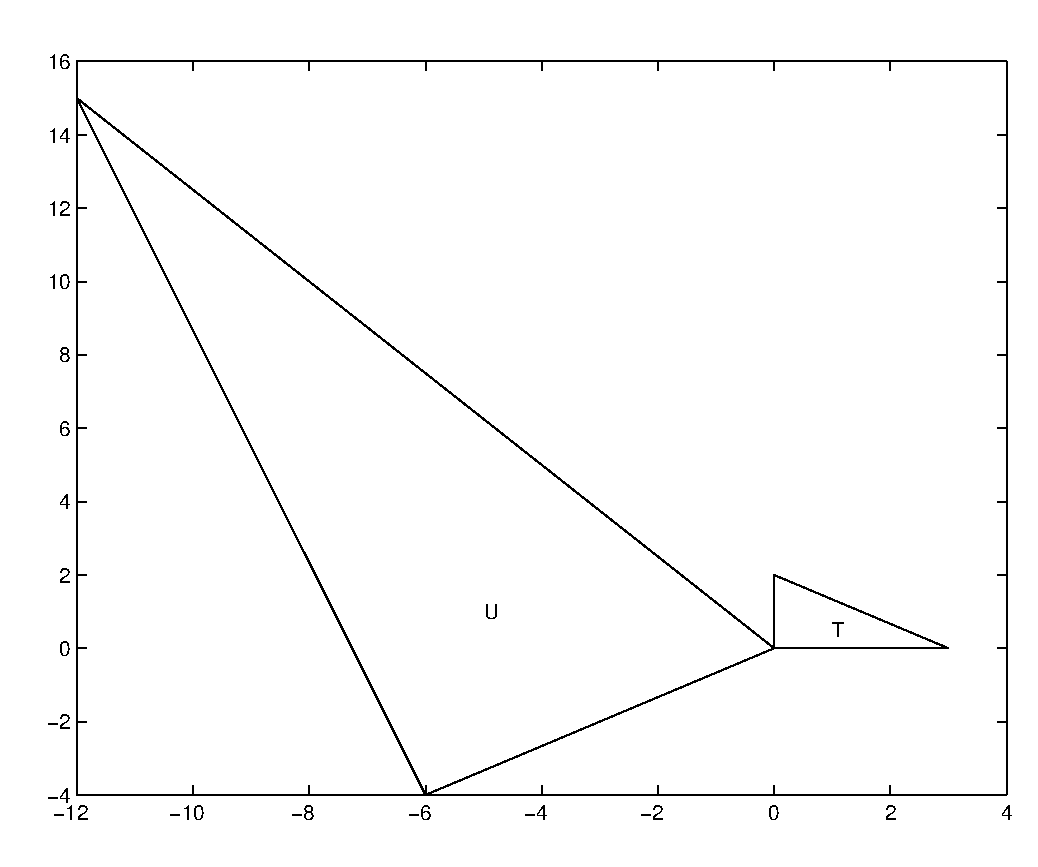
\psfig{file=exfigure/7-8-3.eps,width=3.0in}}
	\exercap{c7.8.3}
\end{figure}

\exer{c7.8.4A}
The general system of linear equations in two unknowns is:
\begin{eqnarray*}
a_{11}x_1+a_{12}x_2 & = & b_1\\
a_{21}x_1+a_{22}x_2 & = & b_2.
\end{eqnarray*}
Subtract $a_{11}$ times the $2^{nd}$ equation from $a_{21}$ times the $1^{st}$ 
equation to eliminate $x_1$ and obtain
\[
(a_{21}a_{12}-a_{11}a_{22})x_2 = (a_{21}b_1-a_{11}b_2).
\]
Therefore
\[
x_2 =  \frac{a_{21}b_1-a_{11}b_2}{a_{21}a_{12}-a_{11}a_{22}}
= \frac{\det(B_2)}{\det(A)}.
\]
A similar argument works for $x_1$.

\exer{c7.8.4B}  \ans  $x=\frac{13}{19}$.

\soln By Cramer's rule (see \Ref{E:cramer}),
\[
x = \det\mattwo{2}{3}{1}{-5}\left/\det\mattwo{2}{3}{3}{-5}=\frac{-13}{-19}\right..
\]
 

\exer{c7.8.4C} \ans  $y=\frac{29}{11}$.

\soln By Cramer's rule (see \Ref{E:cramer}),
\[
y = \det\mattwo{4}{-1}{1}{7}\left/\det\mattwo{4}{-3}{1}{2}=\frac{29}{11}\right..
\]

\exer{c4.9.9}
A randomly selected $2 \times 2$ matrix is almost always invertible.
A matrix will fail to be invertible only if the determinant of the
matrix is $0$, which is seldom the case.

\exer{c3.8.AA} \ans The matrix $A$ is invertible and $\det(A) = 4$.

\soln Figure~\ref{c3.8.AA} shows the {\tt map} output for this matrix.
The area of the square resulting from the map is $4$, so $|\det(A)| = 4$.

\exer{c3.8.AB} \ans The matrix $A$ is not invertible and $\det(A) = 0$.

\soln Figure~\ref{c3.8.AB} shows the {\tt map} output for this matrix.
The square is mapped to a line, whose area is $0$, so $|\det(A)| = 0$.

\exer{c3.8.AC} \ans The matrix $A$ is not invertible and $\det(A) = 0$.

\soln Figure~\ref{c3.8.AC} shows the {\tt map} output for this matrix.
The square is mapped to a line, whose area is $0$, so $|\det(A)| = 0$.

\newpage
\exer{c3.8.AB} \ans The matrix $A$ is invertible and $\det(A) = 1$.

\soln Figure~\ref{c3.8.AD} shows the {\tt map} output for this matrix.
The result of the map is another square of area $1$, so $|\det(A)| = 1$.

\begin{figure}[htb]
                       \centerline{%
                       \psfig{file=exfigure/3-8-AA.eps,width=1.35in}
                       \psfig{file=exfigure/3-8-AB.eps,width=1.35in}
                       \psfig{file=exfigure/3-8-AC.eps,width=1.35in}
                       \psfig{file=exfigure/3-8-AD.eps,width=1.35in}}
        \centerline{Figure~\ref{c3.8.AA}\hspace{0.8in}
        Figure~\ref{c3.8.AB}\hspace{0.8in}Figure~\ref{c3.8.AC}
        \hspace{0.8in}Figure~\ref{c3.8.AD}}
\end{figure}
\end{document}
